\documentclass{beamer}
\usepackage{lmodern}
\usepackage[utf8]{inputenc}


%\usepackage[latin1]{inputenc}
\usepackage[english]{babel}
\usepackage{amsmath}
\usepackage{cases}
\usepackage[makeroom]{cancel}
\usepackage{amsmath,tabu}
\usepackage[fleqn]{mathtools}
\usepackage[fleqn]{amsmath}
\usepackage{bm}
\usepackage{tikz}
\usepackage{enumitem}
\usepackage{wrapfig}
\usepackage{graphicx}
\usepackage{siunitx}
\usepackage{microtype}
\usepackage{array,tabularx}
\usepackage{float}
\usepackage{booktabs}
\usepackage{import}
\usepackage{cases}
\usepackage{graphicx,subfigure}
\usepackage{myUnitOfMeasure}
%\usepackage{myThermodynamics}
\usepackage{myMath}
\usepackage{mathtools}
\usepackage{gensymb}
\usepackage{xcolor}
\usepackage{url}
\usepackage{tabularx}
\usepackage{ltablex}
\usepackage{booktabs}
\usepackage{float}
\usepackage{listings}
\restylefloat{table} % with H force table position

\usepackage{enumerate}
\usepackage{multimedia}

% usefull for ltablex to split long tables in many pages
\keepXColumns

\DeclarePairedDelimiter\abs{\lvert}{\rvert}%

%\newcommand{\Fy}[1]{\text{F}_{y_{#1}}}

%\newcommand{\diameter}{\oslash}

%\newcommand{\todo}{\colorbox{cyan!60}{TODO}}

\renewcommand{\thesubsection}{\thesection.\arabic{subsection}}

\renewcommand{\arraystretch}{1.4}

\newcommand{\variable}[1]{\textcolor{blue}{#1}}

\newcommand{\paramtext}[1]{\textcolor{black!30!green}{#1}}

\newcommand{\terminal}[1]{\textcolor{black!30!cyan}{#1}}

\newcommand{\todo}{\colorbox{cyan!60}{TODO}}

\newcommand{\nut}{\nu_\text{T}}

\newcommand{\foam}[1]{{\ttfamily #1}}


\lstset{
	basicstyle=\fontsize{11}{13}\selectfont\ttfamily,
    frame=tb, % draw a frame at the top and bottom of the code block
    tabsize=4, % tab space width
    showstringspaces=false, % don't mark spaces in strings
    numbers=left, % display line numbers on the left
    commentstyle=\color{black!50!green}, % comment color
    keywordstyle=\color{blue!50!cyan}, % keyword color
    stringstyle=\color{black!30!red} % string color
}



\newcommand{\fakecaption}{%
  \vskip0.5\baselineskip
  \refstepcounter{table}%
  \tablename\ \thetable%
}


\usetheme{polimix}
 
\title[MRL TURBINE]{MRL TURBINE SIMULATION}
\subtitle{MODELLING TECHNIQUES FOR FLUID MACHINES}

\author[AR MB MB AC]{Andrea Rossi \and Marco Bonasegale \and Marco Belloli \and Alberto Casali}

\supervisor{Supervisor}{Gianluca Montenegro \quad Giacomo Persico}

\coadvisor{Co-Advisor}{Augusto Della Torre}
%\date[06/07/2018]{July 2018}
\date{}
\begin{document}

%%%%%%%%%%%%%%%%%%%%%%%%%%%%%%%%%%%%%%%%%%%%%%%%%%%%%%%%%%%%%%%%%%%%%%%%%%%%%%%%%%%%%%%%%%%%%%%%%%%%%%%%%%%%%%%%%%%%

\begin{frame}
\titlepage
\end{frame}

\addtocounter{framenumber}{-1}

%%%%%%%%%%%%%%%%%%%%%%%%%%%%%%%%%%%%%%%%%%%%%%%%%%%%%%%%%%%%%%%%%%%%%%%%%%%%%%%%%%%%%%%%%%%%%%%%%%%%%%%%%%%%%%%%%%%%

%\begin{frame}
%\frametitle{Sommario}
%\tableofcontents
%\end{frame}
%







%%%%%%%%%%%%%%%%%%%%%%%%%%%%%%%%%%%%%%%%%%%%%%%%%%%%%%%%%%%%%%%%%%%%%%%%%%%%%%%%%%%%%%%%%%%%%%%%%%%%%%%%%%%%%%%%%%%
\section{Introduction}

\begin{frame}
\frametitle{Introduction}
The MRL (Momentum Reversal and Lift) Turbine is a hydraulic machine.
Problem data are:
\begin{itemize}
\item[$\cdot$] Inlet flow velocity of $1\ms$;
\item[$\cdot$] shaft rotational speed of $100 \, \text{rpm}$;
\item[$\cdot$] blades counter rotational speed of $50 \, \text{rpm}$;
\item[$\cdot$] geometry of the problem.
\end{itemize}

\begin{center}
\begin{figure}
\includegraphics[width=0.9\textwidth]{images/flow.png} 

\end{figure}
\end{center}


\end{frame}

%%%%%%%%%%%%%%%%%%%%%%%%%%%%%%%%%%%%%%%%%%%%%%%%%%%%%%%%%%%%%%%%%%%%%%%%%%%%%%%%%%%%%%%%%%%%%%%%%%%%%%%%%%%%%%%%%%%
\section{In class work}

%%%%%%%%%%%%%%%%%%%%%%%%%%%%%%%%%%%%%%%%%%%%%%
\begin{frame}
\frametitle{In class work - mesh generation}
The steps for the mesh generation are:
\begin{itemize}
\item[$\cdot$] \foam{surfaceTransformPoints} to scale of the STL files;
\item[$\cdot$] \foam{blockMesh} and \foam{snappyHexMesh} of each regions and blades;
\item[$\cdot$] \foam{mergeMesh} to marge the 5 previous regions;
\item[$\cdot$] \foam{extrudeMesh} to reconstruct a 2D mesh;
\item[$\cdot$] \foam{refineWallLayer} to reduce layers size near the blades.
\end{itemize}

\begin{figure}[H]
\centering
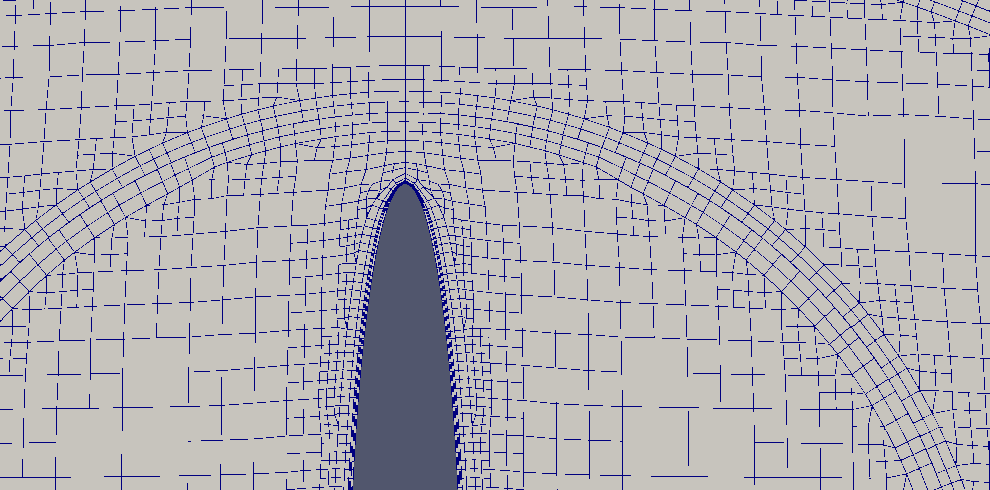
\includegraphics[height=4cm]{images/inclass/mesh40.pdf}
\end{figure}

\end{frame}

%%%%%%%%%%%%%%%%%%%%%%%%%%%%%%%%%%%%%%%%%%%%%%
\begin{frame}
\frametitle{In class work - the boundaries}

\textbf{Inlet} \quad velocity is fixed to $1\ms$ while all the other quatities are calculated according to the physics of the simulation.
\\
\textbf{Outlet} \quad relative pressure is fixed to $0 \,\text{m}^2/\text{s}^2$ (atmosferic pressure) while all the others are free to change according to upstream evolution.
\\
\textbf{Upper surface} \quad relative pressure is fixed to $0 \,\text{m}^2/\text{s}^2$ (atmosferic pressure) while all the others are free to change according to the flow evolution.
\\
\textbf{Bottom wall} \quad velocity is set to no slip condition to mimic adherence and so boundary layer evolution. Pressure is set to \foam{zeroGradient}, typical condition in B.L. All the others are free.
\\\textbf{Blades} \quad a similar no slip condition for moving walls is applied for the velocity. B.L. is isobaric without gradient of pressure. All the others depends on flow solution.

\end{frame}


%%%%%%%%%%%%%%%%%%%%%%%%%%%%%%%%%%%%%%%%%%%%%%
\begin{frame}
\frametitle{In class work - the simulation results}

\begin{figure}[H]
\subfigure[Pressure at 2.4]{\includegraphics[width=5cm]{images/inclass/{pfield2.4sec}.png}}
\hfill
\subfigure[Velocity at 2.4]{\includegraphics[width=5cm]{images/inclass/{velocityfield2.4sec}.png}}
\end{figure}

\begin{table}[H]
\centering
\begin{tabular}{lr}
\toprule
Power (Pressure) [W]     & $\round{4.84602561871}$   \\ \midrule
Power (Shear stress) (W) & $\round{-0.253811271949}$ \\
Power (Total) [W]        & $\round{4.59221434676}$   \\ \bottomrule
\end{tabular}
\caption{Mean power between 1.8 and 2.4}
\label{table:inclass-power}
\end{table}

\end{frame}

%%%%%%%%%%%%%%%%%%%%%%%%%%%%%%%%%%%%%%%%%%%%%%
%%%%%%%%%%%%%%%%%%%%%%%%%%%%%%%%%%%%%%%%%%%%%%
\section{Mesh sensitivity analysis}

%%%%%%%%%%%%%%%%%%%%%%%%%%%%%%%%%%%%%%%%%%%%%%
\begin{frame}
\frametitle{Mesh sensitivity analysis}

We have performed the sensibility analysis with two different kind of grid:
\begin{itemize}
\item[$\cdot$] mesh without refinement region around blades;
\item[$\cdot$] mesh with refinement regiorn around blades.
\end{itemize}

\begin{figure}
\subfigure[Mesh without refinement region]{\includegraphics[width=5cm]{images/meshsensitivity/mesh120-blade0-noregion.png}}
\hfill
\subfigure[Mesh with refinement region]{\includegraphics[width=5cm]{images/meshsensitivity/mesh120-blade0-region.png}}
\end{figure}

\end{frame}


%%%%%%%%%%%%%%%%%%%%%%%%%%%%%%%%%%%%%%%%%%%%%%
\begin{frame}
\frametitle{Mesh sensitivity analysis}

We have improved the number of cells acting on the refinement of the y axis.
We have started from 20 cells and have arrived to 160 cells.
\begin{table}[H]
\centering
\begin{tabular}{lrr}
\toprule
         & Without region & With region \\ \midrule
Mesh 20  & 10328          & 9696        \\
Mesh 40  & 24066          & 24021       \\
Mesh 60  & 40462          & 42508       \\
Mesh 80  & 58877          & 64293       \\
Mesh 120 & 103384         & 120614      \\
Mesh 160 & 156791         & 160547      \\ \bottomrule
\end{tabular}
\end{table}

\end{frame}




























\begin{frame}
\frametitle{Title B1}
\begin{itemize}
\addtolength{\itemsep}{.2cm}
\item Lorem ipsum dolor sit amet, consectetur adipiscing elit.
\item Nulla id ex ornare, gravida nisi in, ornare risus.
  \begin{itemize}
    \addtolength{\itemsep}{.1cm}
  \item[1.] Aenean eu posuere purus.
  \item[2.] Etiam maximus convallis libero, ac venenatis nunc sagittis nec.
  \end{itemize}
\item Suspendisse orci ex, pharetra vitae aliquam ac, rutrum in dui.
\end{itemize}

\end{frame}

%%%%%%%%%%%%%%%%%%%%%%%%%%%%%%%%%%%%%%%%%%%%%%%%%%%%%%%%%%%%%%%%%%%%%%%%%%%%%%%%%%%%%%%%%%%%%%%%%%%%%%%%%%%%%%%%%%%

\begin{frame}
\frametitle{Title B2}

\begin{theorem}[Th. Name]
\label{thlabel} This is a theorem
\begin{itemize}
\item Property 1;
\item Property 2.
\end{itemize}
\end{theorem}

\pause

\textit{Proof. }
\begin{align}
    a + b & = c \\
    a & = c - b \\
    answer & = 42
\end{align}
\qed

\pause

\begin{proof}
Another proof style.
\end{proof}

\end{frame}

%%%%%%%%%%%%%%%%%%%%%%%%%%%%%%%%%%%%%%%%%%%%%%%%%%%%%%%%%%%%%%%%%%%%%%%%%%%%%%%%%%%%%%%%%%%%%%%%%%%%%%%%%%%%%%%%%%%%
\section{Section C}

\begin{frame}
\frametitle{Title C1}

\begin{columns}[t, onlytextwidth]
\column{.33\textwidth}
First column.\\
\onslide<3>{\bigskip Appears with third column}
\pause{}
\column{.33\textwidth}
Second column.
\pause
\column{.33\textwidth}
Third column.
\end{columns}

\end{frame}

%%%%%%%%%%%%%%%%%%%%%%%%%%%%%%%%%%%%%%%%%%%%%%%%%%%%%%%%%%%%%%%%%%%%%%%%%%%%%%%%%%%%%%%%%%%%%%%%%%%%%%%%%%%%%%%%%%%%

\begin{frame}
\frametitle{Title C2}


\centering
Image:\\
\bigskip\bigskip
\includegraphics[height=2cm]{style_img/20090504_Politecnico_0006_02}

\end{frame}

%%%%%%%%%%%%%%%%%%%%%%%%%%%%%%%%%%%%%%%%%%%%%%%%%%%%%%%%%%%%%%%%%%%%%%%%%%%%%%%%%%%%%%%%%%%%%%%%%%%%%%%%%%%%%%%%%%%%

\begin{frame}
\frametitle{Title C3}


%\begin{enumerate}
% \item lorem
% \item Ipsus
% \begin{enumerate}
%    \item sub1
%    \item sub3
%    \begin{enumerate}
%      \item sub4
%      \item sub5
%    \end{enumerate}
% \end{enumerate}
%\end{enumerate}


\end{frame}

%%%%%%%%%%%%%%%%%%%%%%%%%%%%%%%%%%%%%%%%%%%%%%%%%%%%%%%%%%%%%%%%%%%%%%%%%%%%%%%%%%%%%%%%%%%%%%%%%%%%%%%%%%%%%%%%%%

\begin{frame}
\frametitle{Video}
\movie[width=\textwidth, height = 0.8\paperheight, poster, autostart, borderwidth=1pt]{}{video/test.mp4} 

\end{frame}


\end{document} 
